\documentclass[12pt]{article}

\usepackage{sbc-template}
\usepackage[utf8]{inputenc}
\usepackage[T1]{fontenc}
\usepackage[brazil]{babel}
\usepackage{graphicx,url}
\usepackage{amsmath,amssymb}
\usepackage{icomma}
\usepackage{booktabs}
\usepackage{algorithm}
\usepackage[noend]{algpseudocode}

% Pseudocódigo em português
\floatname{algorithm}{Algoritmo}
\algrenewcommand\algorithmicrequire{\textbf{Entrada:}}
\algrenewcommand\algorithmicensure{\textbf{Saída:}}
\algrenewcommand\algorithmicwhile{\textbf{enquanto}}
\algrenewcommand\algorithmicdo{\textbf{faça}}
\algrenewcommand\algorithmicfor{\textbf{para}}
\algrenewcommand\algorithmicif{\textbf{se}}
\algrenewcommand\algorithmicthen{\textbf{então}}
\algrenewcommand\algorithmicelse{\textbf{senão}}
\algrenewcommand\algorithmicreturn{\textbf{retorne}}

% posicionamento de figuras e tabelas mais flexível
\renewcommand{\topfraction}{0.9}
\renewcommand{\bottomfraction}{0.8}
\renewcommand{\textfraction}{0.07}
\renewcommand{\floatpagefraction}{0.8}
\setcounter{topnumber}{3}
\setcounter{bottomnumber}{2}
\setcounter{totalnumber}{4}

\newcommand{\x}{\mathbf{x}}
\newcommand{\vv}{\mathbf{v}}
\newcommand{\uu}{\mathbf{u}}

\sloppy
\raggedbottom % evita espaços verticais esticados nas páginas com figuras

\title{Uma introdução à Evolução Diferencial}

\author{[Nome do Autor]\inst{1}}

\address{Programa de Pós-Graduação em Informática (PPGI)\\
  Universidade Federal do Espírito Santo (UFES) -- Vitória, ES -- Brasil
  \email{[email]}
}

\begin{document}

\maketitle

\begin{abstract}
  Differential Evolution (DE) is a population-based metaheuristic for global
  optimization over continuous spaces, proposed by Storn and Price in 1995. New
  candidate solutions are built by adding the scaled difference between two
  population members to a third one, followed by binomial crossover and a
  greedy one-to-one selection. This paper reviews the origin and main variants
  of DE, describes the classic DE/rand/1/bin algorithm and how it balances
  exploration and exploitation, and illustrates it on the two-dimensional
  Rastrigin function, a multimodal benchmark with 121 local minima.
\end{abstract}

\begin{resumo}
  A Evolução Diferencial (ED) é uma meta-heurística populacional para
  otimização global em espaços contínuos, proposta por Storn e Price em 1995.
  Novas soluções candidatas são geradas somando a um membro da população a
  diferença ponderada entre outros dois, seguida de um cruzamento binomial e
  de uma seleção gulosa um a um. Este artigo apresenta a origem e as principais
  variantes da ED, descreve o algoritmo clássico DE/rand/1/bin e o modo como
  ele equilibra diversificação e intensificação, e o ilustra na função de
  Rastrigin em duas dimensões, um problema multimodal com 121 mínimos locais.
\end{resumo}

% =============================================================================
\section{Introdução}
% =============================================================================

Muitos problemas de engenharia e ciência podem ser formulados como a
minimização de uma função objetivo $f:\mathbb{R}^D \to \mathbb{R}$ de variáveis
contínuas. Quando $f$ é não linear, não diferenciável ou multimodal, métodos de
gradiente e buscas diretas locais, como a de Nelder e Mead, tendem a parar no
primeiro mínimo local encontrado, pois só aceitam movimentos que melhoram a
solução corrente \cite{storn1997}. Meta-heurísticas populacionais, como os
algoritmos genéticos e as estratégias evolutivas, reduzem esse risco ao manter
várias soluções ao mesmo tempo.

A Evolução Diferencial (ED, ou DE, do inglês \emph{Differential Evolution}) foi
proposta por Rainer Storn e Kenneth Price em um relatório técnico do
International Computer Science Institute, em Berkeley \cite{storn1995}. O
método surgiu das tentativas de Price de resolver um problema de ajuste de
polinômios de Chebyshev proposto por Storn \cite{das2011}. Em 1996, a ED
participou da primeira competição internacional de otimização evolutiva
(1st ICEO, durante a conferência IEEE ICEC'96) e foi o algoritmo evolutivo mais
rápido entre os inscritos
\cite{price1996iceo}. No ano seguinte, o artigo publicado no
\emph{Journal of Global Optimization} consolidou o método: comparada a
variantes de recozimento simulado, a outros algoritmos evolutivos e a um método
de equações diferenciais estocásticas em três conjuntos de funções de teste, a
ED exigiu menos avaliações da função objetivo na maioria dos casos
\cite{storn1997}. Em 2005, os autores reuniram a teoria e a prática do método
em um livro \cite{price2005}.

O estado da arte concentra-se na adaptação automática dos parâmetros de
controle e das estratégias de mutação. O jDE codifica $F$ e $CR$ em cada
indivíduo e os deixa evoluir junto com a solução \cite{brest2006}; o SaDE
escolhe entre várias estratégias de mutação conforme o sucesso recente de cada
uma \cite{qin2009}; o JADE introduziu a mutação \emph{current-to-pbest} com um
arquivo externo de soluções descartadas \cite{zhang2009}; o SHADE adapta $F$ e
$CR$ a partir de uma memória histórica de sucessos \cite{tanabe2013}; e o
L-SHADE, que acrescenta a redução linear do tamanho da população, venceu a
competição de otimização mono-objetivo do IEEE CEC 2014 \cite{tanabe2014}.
Revisões abrangentes dessas variantes são apresentadas em
\cite{das2011} e \cite{das2016}.

Entre as aplicações da ED estão o projeto de filtros digitais
\cite{storn1996iir}, eletromagnetismo, sistemas de potência, engenharia
química, projeto mecânico e aprendizado de máquina
\cite{das2011,das2016,cornell}. A Seção~\ref{sec:definicao} descreve o
algoritmo, suas variantes e parâmetros; a Seção~\ref{sec:aplicacao} aplica a
ED à função de Rastrigin; e a Seção~\ref{sec:conclusoes} apresenta as
conclusões.

% =============================================================================
\section{Definição e descrição da meta-heurística}\label{sec:definicao}
% =============================================================================

A ED trabalha com uma população de $NP$ vetores de parâmetros
$D$-dimensionais, $\x_{i,G}$, $i = 1, \dots, NP$, em que $G$ indica a geração.
O tamanho da população não muda durante a execução. A população inicial é
sorteada com distribuição uniforme dentro dos limites de cada variável,
$x_{j,i,0} = x_j^{\min} + \mathrm{rand}_j(0,1)\,(x_j^{\max} - x_j^{\min})$,
de forma a cobrir todo o espaço de busca \cite{storn1997,baeldung}. A cada
geração, cada vetor da população assume o papel de \emph{vetor-alvo} e passa
por três operações: mutação, cruzamento e seleção.

\textbf{Mutação.} Para cada vetor-alvo $\x_{i,G}$, gera-se um \emph{vetor
mutante} somando a um vetor-base a diferença ponderada entre dois outros
membros da população:
\begin{equation}
  \vv_{i,G+1} = \x_{r_1,G} + F \cdot \left(\x_{r_2,G} - \x_{r_3,G}\right),
  \label{eq:mutacao}
\end{equation}
em que $r_1, r_2, r_3 \in \{1, \dots, NP\}$ são índices sorteados, distintos
entre si e diferentes de $i$ (por isso $NP \ge 4$), e $F > 0$ é o
\emph{fator de escala}, que controla a amplitude da perturbação. Assim, a
direção e o tamanho do passo vêm das diferenças entre os próprios membros da
população, e não de uma distribuição fixa, como nas estratégias evolutivas.

\textbf{Cruzamento.} Para aumentar a diversidade, o mutante é combinado com o
alvo, coordenada a coordenada, formando o \emph{vetor experimental}
$\uu_{i,G+1}$:
\begin{equation}
  u_{j,i,G+1} =
  \begin{cases}
    v_{j,i,G+1}, & \text{se } \mathrm{rand}_j \le CR \text{ ou } j = j_{rand},\\
    x_{j,i,G},   & \text{caso contrário},
  \end{cases}
  \qquad j = 1, \dots, D,
  \label{eq:cruzamento}
\end{equation}
em que $\mathrm{rand}_j \in [0,1]$ é sorteado para cada coordenada,
$CR \in [0,1]$ é a \emph{constante de cruzamento} e $j_{rand}$ é um índice
sorteado que garante que ao menos uma coordenada venha do mutante. O número de
coordenadas herdadas do mutante segue aproximadamente uma distribuição
binomial, daí o nome \emph{cruzamento binomial}.

\textbf{Seleção.} O vetor experimental compete apenas com o seu próprio alvo,
em uma seleção gulosa:
\begin{equation}
  \x_{i,G+1} =
  \begin{cases}
    \uu_{i,G+1}, & \text{se } f(\uu_{i,G+1}) < f(\x_{i,G}),\\
    \x_{i,G},    & \text{caso contrário}.
  \end{cases}
  \label{eq:selecao}
\end{equation}
Assim, ocorrem $NP$ competições por geração e o valor de $f$ associado a cada
posição da população nunca piora. O Algoritmo~\ref{alg:de} resume o método.
Como no pseudocódigo original \cite{storn1997}, a nova população é montada
separadamente e só substitui a atual ao final da geração.

\begin{algorithm}[!tb]
\caption{Evolução Diferencial clássica (DE/rand/1/bin)}\label{alg:de}
\begin{algorithmic}[1]
\Require $f$, limites $[\x^{\min}, \x^{\max}]$, $NP \ge 4$, $F$, $CR$, $G_{\max}$
\State Sortear $\x_{i,0}$ uniformemente nos limites e avaliar $f(\x_{i,0})$, $i = 1,\dots,NP$
\For{$G = 0, 1, \dots, G_{\max}-1$}
  \For{$i = 1, \dots, NP$}
    \State Sortear $r_1 \ne r_2 \ne r_3 \ne i$ em $\{1,\dots,NP\}$ e $j_{rand}$ em $\{1,\dots,D\}$
    \State $\vv \gets \x_{r_1,G} + F\,(\x_{r_2,G} - \x_{r_3,G})$ \Comment{mutação}
    \State $u_j \gets v_j$ se $\mathrm{rand}_j \le CR$ ou $j = j_{rand}$; senão $u_j \gets x_{j,i,G}$ \Comment{cruzamento}
    \State $\x_{i,G+1} \gets \uu$ se $f(\uu) < f(\x_{i,G})$; senão $\x_{i,G+1} \gets \x_{i,G}$ \Comment{seleção}
  \EndFor
\EndFor
\Ensure o melhor vetor da população final
\end{algorithmic}
\end{algorithm}

\textbf{Variantes.} Storn e Price propuseram a notação DE/$x$/$y$/$z$ \cite{storn1997},
em que $x$ indica o vetor-base (\emph{rand}, um vetor aleatório, ou
\emph{best}, o melhor da população), $y$ é o número de vetores diferença e $z$ é
o tipo de cruzamento (\emph{bin}, binomial, ou \emph{exp}, exponencial, que
copia um bloco contíguo de coordenadas). O esquema das
Equações~\ref{eq:mutacao}--\ref{eq:selecao} é o DE/rand/1/bin. Outras
variantes comuns são o DE/best/1, com
$\vv = \x_{best} + F(\x_{r_1} - \x_{r_2})$; o DE/best/2, com
$\vv = \x_{best} + F(\x_{r_1} + \x_{r_2} - \x_{r_3} - \x_{r_4})$; e o
DE/current-to-best/1, com
$\vv = \x_i + F(\x_{best} - \x_i) + F(\x_{r_1} - \x_{r_2})$. As variantes que
usam o melhor vetor convergem mais rápido, mas correm mais risco de
convergência prematura em funções multimodais \cite{das2011}.

\textbf{Parâmetros de controle.} Segundo \cite{storn1997}, uma escolha
razoável é $NP$ entre $5D$ e $10D$; $F = 0{,}5$ é um bom valor inicial, e
valores menores que $0{,}4$ ou maiores que $1$ raramente funcionam bem; para
$CR$, $0{,}1$ é uma primeira escolha segura, mas vale testar $0{,}9$ ou $1{,}0$
em busca de uma convergência rápida. Se a população convergir prematuramente,
deve-se aumentar $F$ e/ou $NP$. Valores baixos de $CR$ funcionam bem em funções
separáveis; valores altos, quando as variáveis interagem \cite{das2011}.

\textbf{Diversificação e intensificação.} O equilíbrio entre explorar o espaço
de busca e refinar as boas soluções surge da própria estrutura do algoritmo.
No início, a população está espalhada, os vetores diferença são longos e a
mutação produz saltos grandes (\emph{diversificação}); o vetor-base aleatório
da variante \emph{rand} reforça esse efeito, e a seleção um a um preserva
diversidade, pois cada posição da população forma uma linhagem própria. À
medida que a seleção gulosa descarta as soluções piores, a população se
concentra nas regiões promissoras, as diferenças entre os vetores diminuem e o
passo da mutação encolhe automaticamente (\emph{intensificação}). Em regiões
planas da função ocorre o inverso: as distâncias entre os vetores aumentam, o
que evita um avanço lento \cite{storn1997}. Os parâmetros $F$, $CR$ e $NP$
regulam, respectivamente, a amplitude dos passos, quantas coordenadas mudam e
quanta diversidade é mantida.

\textbf{Exemplo numérico.} A Tabela~\ref{tab:exemplo} e a
Figura~\ref{fig:vetores} mostram uma iteração para um vetor-alvo da população
inicial do experimento da Seção~\ref{sec:aplicacao} ($F = 0{,}5$,
$CR = 0{,}9$). No cruzamento, $\mathrm{rand}_1 = 0{,}374 \le CR$, e a primeira
coordenada veio do mutante; como $\mathrm{rand}_2 = 0{,}987 > CR$ e
$j_{rand} = 1$, a segunda foi herdada do alvo. Como
$f(\uu) = 26{,}770 < f(\x_i) = 31{,}887$, o vetor experimental substitui o alvo
na próxima geração.

\begin{figure}[!tb]
\centering
\begin{minipage}[c]{.46\textwidth}
\centering
\captionsetup{margin=0pt,format=plain,justification=centering}
\captionof{table}{Uma iteração da DE/rand/1/bin para um vetor-alvo da
população inicial ($F = 0{,}5$, $CR = 0{,}9$).}\label{tab:exemplo}
\footnotesize
\setlength{\tabcolsep}{4pt}
\begin{tabular}{lrrr}
\toprule
Vetor & $x_1$ & $x_2$ & $f(\x)$ \\
\midrule
$\x_i$ (alvo)            & $2{,}805$  & $-0{,}626$ & $31{,}887$ \\
$\x_{r_1}$ (base)        & $0{,}559$  & $-4{,}467$ & $59{,}363$ \\
$\x_{r_2}$               & $-2{,}796$ & $1{,}739$  & $28{,}664$ \\
$\x_{r_3}$               & $2{,}643$  & $-1{,}490$ & $45{,}419$ \\
$\x_{r_2} - \x_{r_3}$    & $-5{,}439$ & $3{,}229$  & -- \\
$\vv$ (mutante)          & $-2{,}161$ & $-2{,}852$ & -- \\
$\mathrm{rand}_j$        & $0{,}374$  & $0{,}987$  & -- \\
$\uu$ (experimental)     & $-2{,}161$ & $-0{,}626$ & $26{,}770$ \\
\bottomrule
\end{tabular}
\end{minipage}\hfill
\begin{minipage}[c]{.5\textwidth}
\centering
\captionsetup{margin=0pt,format=plain,justification=centering}
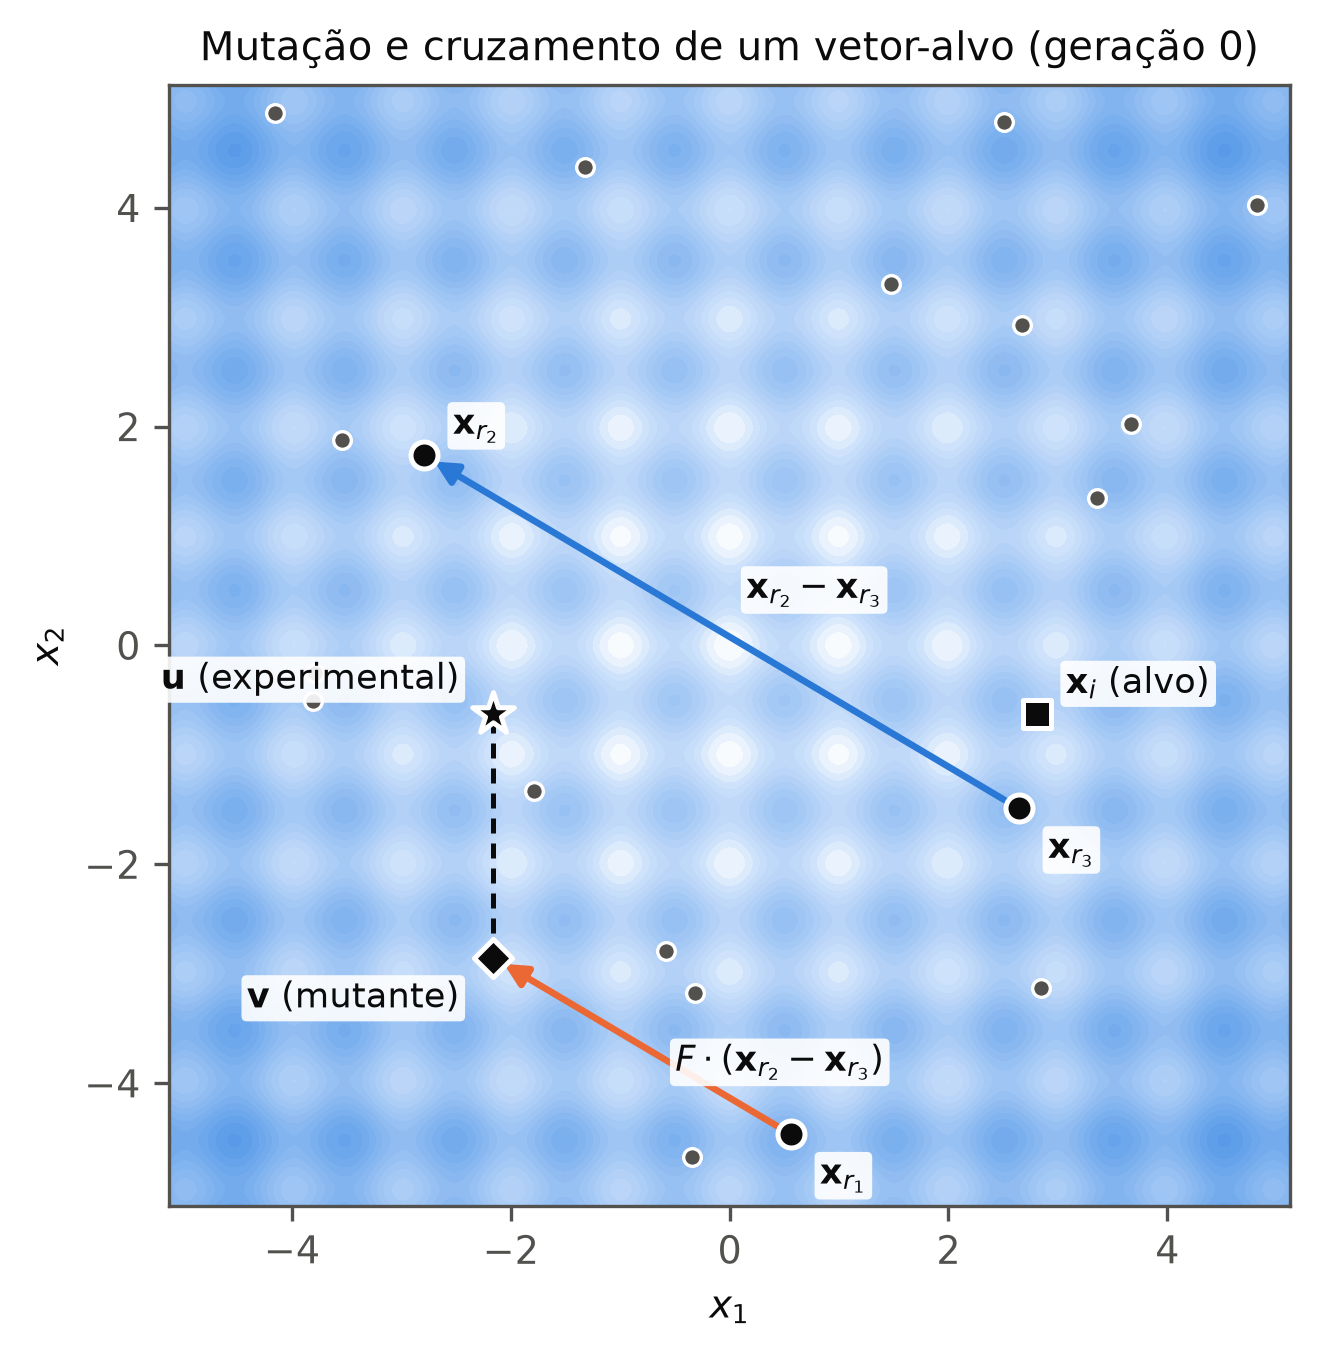
\includegraphics[width=\linewidth]{figuras/mutacao_vetores.png}
\caption{Vetores da Tabela~\ref{tab:exemplo}: diferença (azul), passo
$F(\x_{r_2} - \x_{r_3})$ (laranja) e cruzamento (tracejado).}
\label{fig:vetores}
\end{minipage}
\end{figure}

% =============================================================================
\section{Exemplo de aplicação da meta-heurística}\label{sec:aplicacao}
% =============================================================================

\subsection{O problema}

Para ilustrar o funcionamento da ED, escolheu-se a minimização da função de
Rastrigin,
\begin{equation}
  f(\x) = 10D + \sum_{j=1}^{D} \left[ x_j^2 - 10\cos(2\pi x_j) \right],
  \qquad \x \in [-5{,}12;\ 5{,}12]^D,
  \label{eq:rastrigin}
\end{equation}
com $D = 2$. A função combina uma parábola com uma ondulação cossenoidal
(Figura~\ref{fig:rastrigin}): há um mínimo local perto de cada ponto de
coordenadas inteiras, 121 no domínio, e um único mínimo global,
$f(0,0) = 0$, o que a torna um teste clássico de otimização global. Ela integra
o conjunto de testes de \cite{storn1997}, lá com domínio $[-600, 600]$; aqui
usou-se o domínio usual para permitir visualizar a população.


\subsection{Implementação}

O experimento foi implementado em Python com a classe \texttt{DE} da biblioteca
pymoo, versão 0.6.2 \cite{blank2020}, em um \emph{notebook} Jupyter que também
gera as figuras deste artigo e uma animação da população. A configuração
(Tabela~\ref{tab:parametros}) segue as recomendações da
Seção~\ref{sec:definicao}.

\begin{figure}[!tb]
\centering
\begin{minipage}[c]{.29\textwidth}
\centering
\captionsetup{margin=0pt,format=plain,justification=centering}
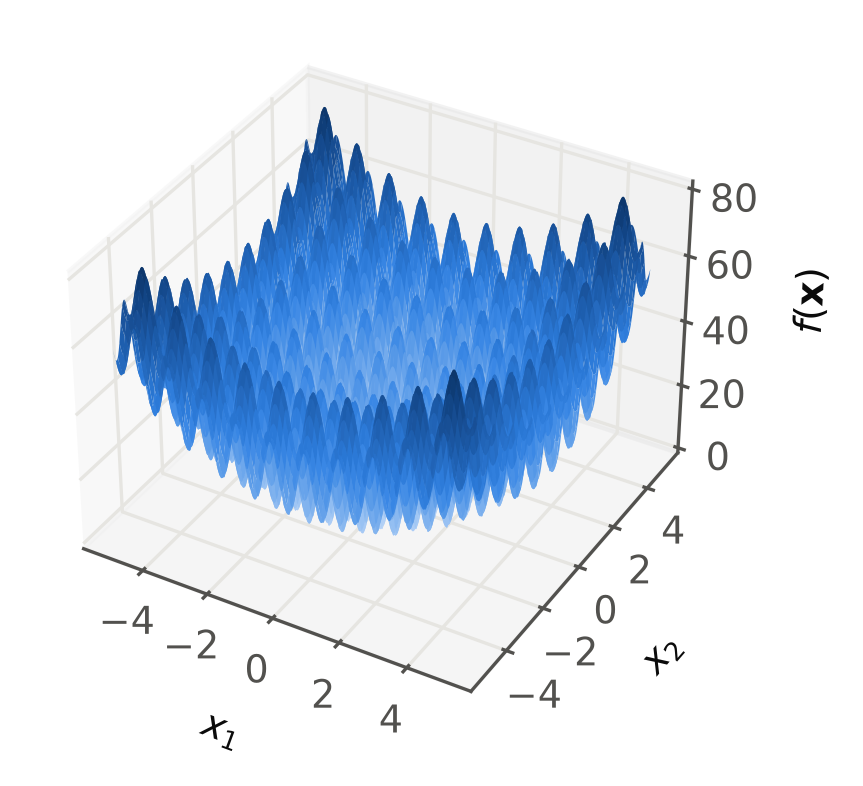
\includegraphics[width=\linewidth]{figuras/rastrigin_3d.png}
\caption{Função de Rastrigin ($D = 2$).}\label{fig:rastrigin}
\end{minipage}\hfill
\begin{minipage}[c]{.69\textwidth}
\centering
\captionsetup{margin=0pt,format=plain,justification=centering}
\captionof{table}{Configuração do experimento.}\label{tab:parametros}
\footnotesize
\setlength{\tabcolsep}{4pt}
\begin{tabular}{lll}
\toprule
Parâmetro & Valor & Argumento no \texttt{DE} do pymoo \\
\midrule
Estratégia      & DE/rand/1/bin      & \texttt{variant="DE/rand/1/bin"} \\
População       & $NP = 20$ ($10D$)  & \texttt{pop\_size=20} \\
Fator de escala & $F = 0{,}5$        & \texttt{F=0.5, jitter=False} \\
Cruzamento      & $CR = 0{,}9$       & \texttt{CR=0.9} \\
Mutação extra   & desligada          & \texttt{prob\_mut=0.0} \\
Gerações        & $G_{\max} = 100$   & \texttt{("n\_gen", 101)} \\
Semente         & 42                 & \texttt{seed=42} \\
\bottomrule
\end{tabular}
\end{minipage}
\end{figure}

Alguns padrões do pymoo diferem da ED clássica e foram alterados: a variante
padrão é a DE/best/1/bin, o $CR$ padrão é $0{,}2$ e, após o cruzamento, a
biblioteca aplica uma mutação polinomial extra (probabilidade $0{,}1$), que foi
desligada por não fazer parte do algoritmo original. No pymoo, uma coordenada
do mutante que sai do domínio é sorteada entre o vetor-base e o limite violado,
e o papel de $j_{rand}$ é cumprido sorteando uma coordenada do mutante só quando
nenhuma passa no teste $\mathrm{rand}_j \le CR$. Como a inicialização conta
como primeira geração, 101 gerações do pymoo equivalem a 100 gerações da ED, ou
$NP \times 101 = 2020$ avaliações de $f$.

\subsection{Resultados}

A Figura~\ref{fig:populacao} mostra a população em quatro instantes da
execução. Na geração 0, os 20 indivíduos estão espalhados pelo domínio e ocupam
19 bacias de atração diferentes (contadas pelo ponto de coordenadas inteiras
mais próximo de cada indivíduo). Na geração 5, o melhor valor caiu de $25{,}0$
para $3{,}37$, mas a população ainda ocupa 14 bacias; na geração 15, ela se
concentra perto da origem (12 bacias) e, na geração 35, restam 3. A partir da
geração 42, todos os indivíduos estão na bacia do mínimo global e o restante da
execução é de intensificação: na geração 100, a melhor solução foi
$\x^* = (-2{,}49 \times 10^{-9};\ -2{,}40 \times 10^{-9})$, com
$f(\x^*) = 3{,}55 \times 10^{-15}$. O limiar $f < 10^{-6}$ foi atingido na
geração 61, após 1240 avaliações de $f$.

\begin{figure}[!tb]
\centering
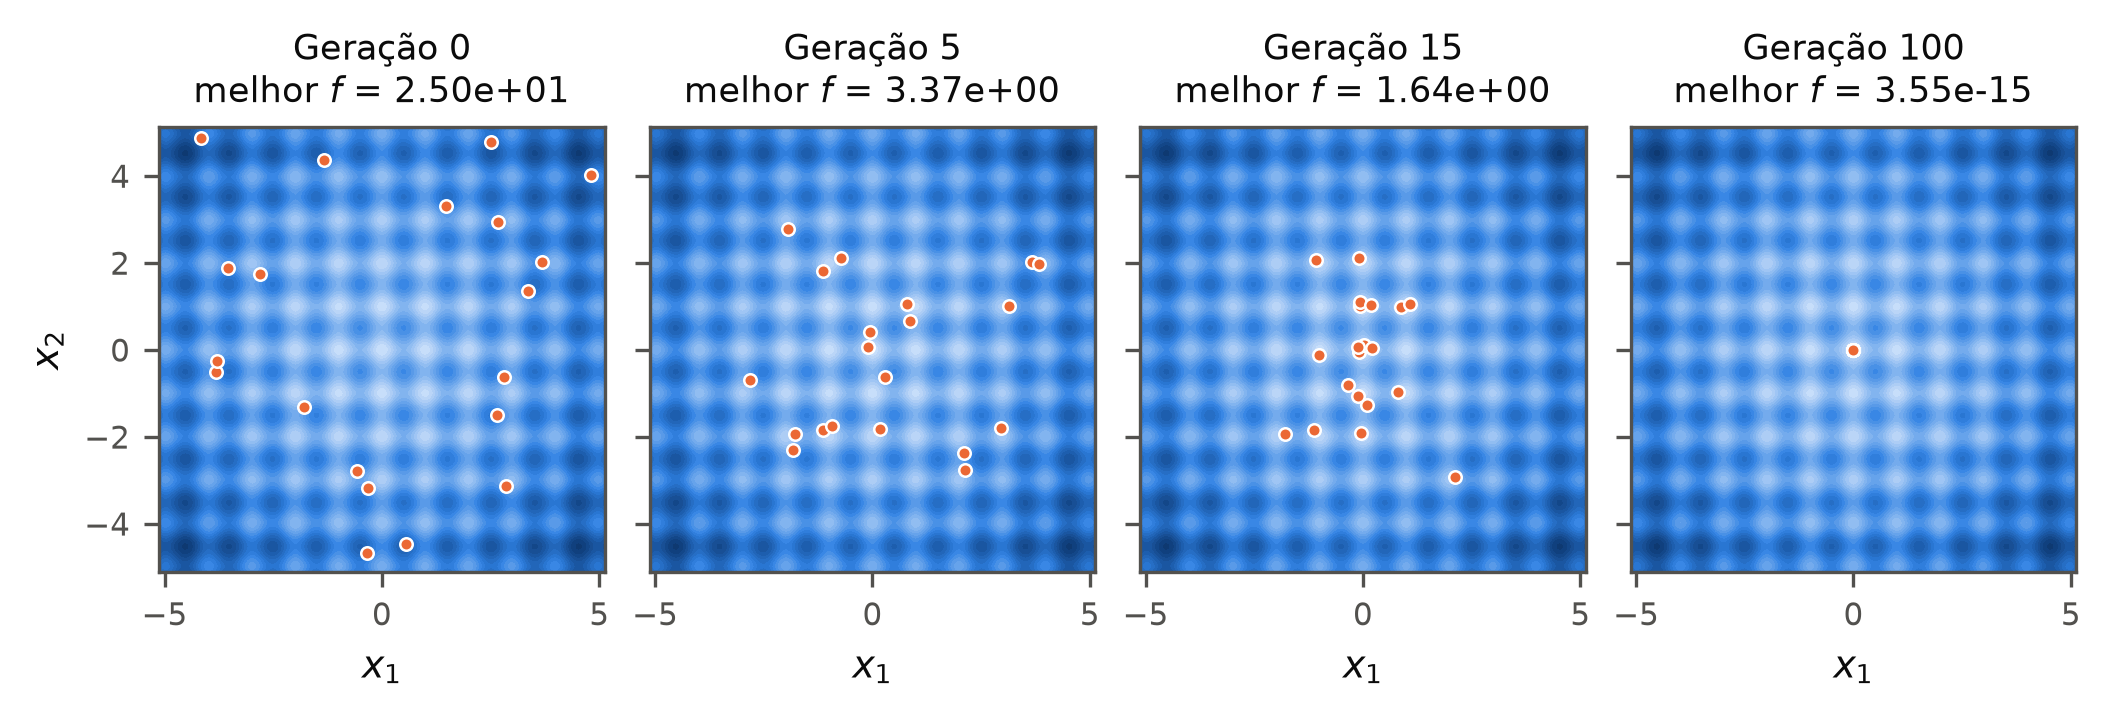
\includegraphics[width=.86\textwidth]{figuras/populacao_geracoes_linha.png}
\caption{População da ED (pontos laranja) nas gerações 0, 5, 15 e 100 sobre as
curvas de nível da função de Rastrigin.}
\label{fig:populacao}
\end{figure}

A Figura~\ref{fig:convergencia} resume a execução. O melhor valor de $f$ cai
em patamares, pois só muda quando algum vetor experimental supera o melhor
indivíduo, enquanto a média da população cai de forma contínua. A dispersão da
população, medida como a distância média dos indivíduos ao centroide, cai de
$4{,}02$ para $1{,}8 \times 10^{-8}$. Como os vetores diferença são formados
pelos próprios indivíduos, essa é também a escala dos passos da mutação, que a
ED reduziu em mais de oito ordens de grandeza sem nenhum parâmetro adicional. A
queda abrupta perto da geração 40 coincide com a eliminação dos últimos
indivíduos que estavam em bacias vizinhas à do mínimo global.

\begin{figure}[!tb]
\centering
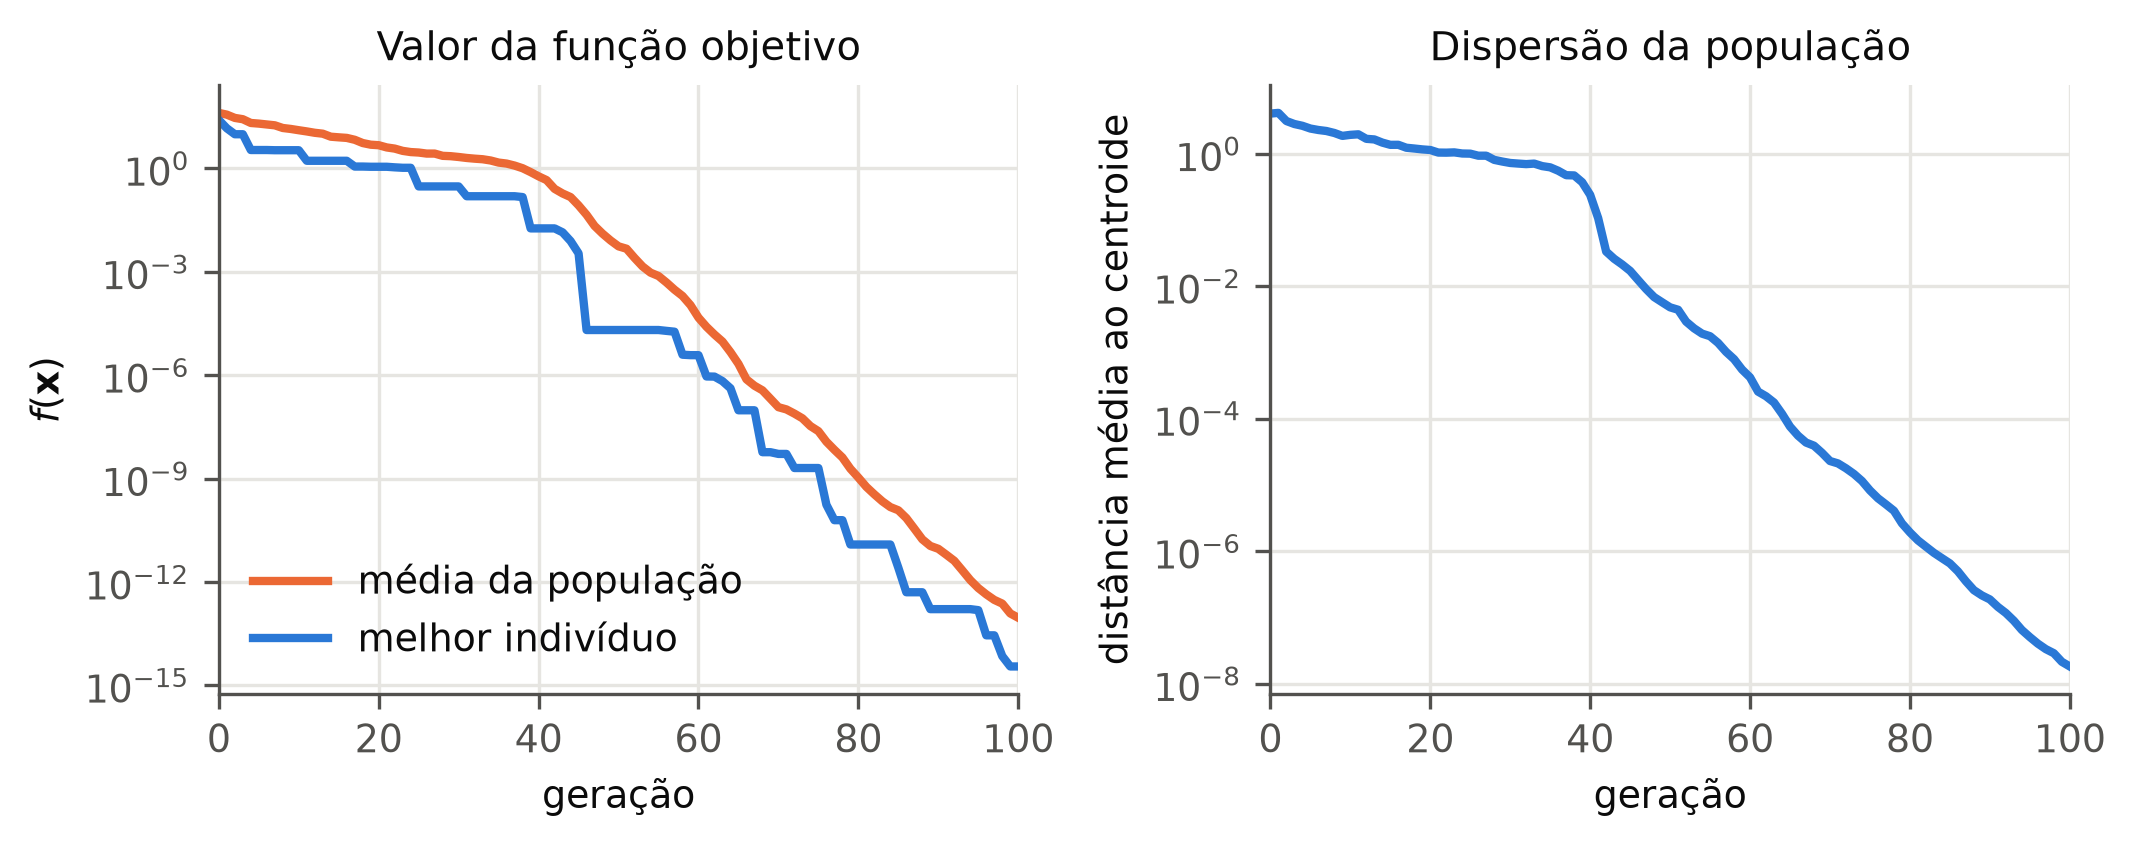
\includegraphics[width=.7\textwidth]{figuras/convergencia.png}
\caption{Convergência da ED na função de Rastrigin: valor de $f$ do melhor
indivíduo e média da população (à esquerda) e dispersão da população (à
direita), em escala logarítmica.}
\label{fig:convergencia}
\end{figure}

% =============================================================================
\section{Principais conclusões}\label{sec:conclusoes}
% =============================================================================

A Evolução Diferencial é uma meta-heurística populacional simples: seu núcleo
cabe em poucas linhas de código e depende de apenas três parâmetros de
controle, para os quais existem boas regras práticas. Ela não exige derivadas,
trata naturalmente problemas multimodais e é fácil de paralelizar. Sua
característica mais marcante é a mutação baseada em vetores diferença, que
ajusta o tamanho do passo à distribuição da população e produz a transição da
diversificação para a intensificação observada na Seção~\ref{sec:aplicacao}, em
que o método encontrou o mínimo global da função de Rastrigin, entre 121
mínimos locais, com 1240 avaliações até atingir $f < 10^{-6}$.

Entre as limitações, o desempenho depende de $F$, $CR$ e da estratégia de
mutação, cuja melhor escolha varia com o problema (o que motivou as variantes
adaptativas), e a população pode estagnar ou convergir prematuramente,
sobretudo se for pequena ou se a variante for gulosa, como a DE/best. A formulação original é voltada a
variáveis contínuas sem restrições: problemas discretos ou com restrições
exigem adaptações, como arredondamento ou funções de penalidade. O custo cresce
com a dimensão, e não há garantia teórica de convergência para o ótimo global.
Por fim, nenhuma meta-heurística é superior a todas as outras em todos os
problemas \cite{wolpert1997}; ainda assim, a simplicidade, a robustez e o bom
desempenho em otimização contínua mantêm a ED entre as meta-heurísticas mais
usadas e estudadas.

\bibliographystyle{sbc}
\bibliography{referencias}

\end{document}
